\section{Metodología de Investigación}

Esta sección se desarrolló en base a los niveles de maduración tecnológica TRL (Technology Readiness Level) ilustrados por el departamento administrativo de ciencia, tecnología e innovación Colciencias.
  

\begin{figure}[H]
    \centering
    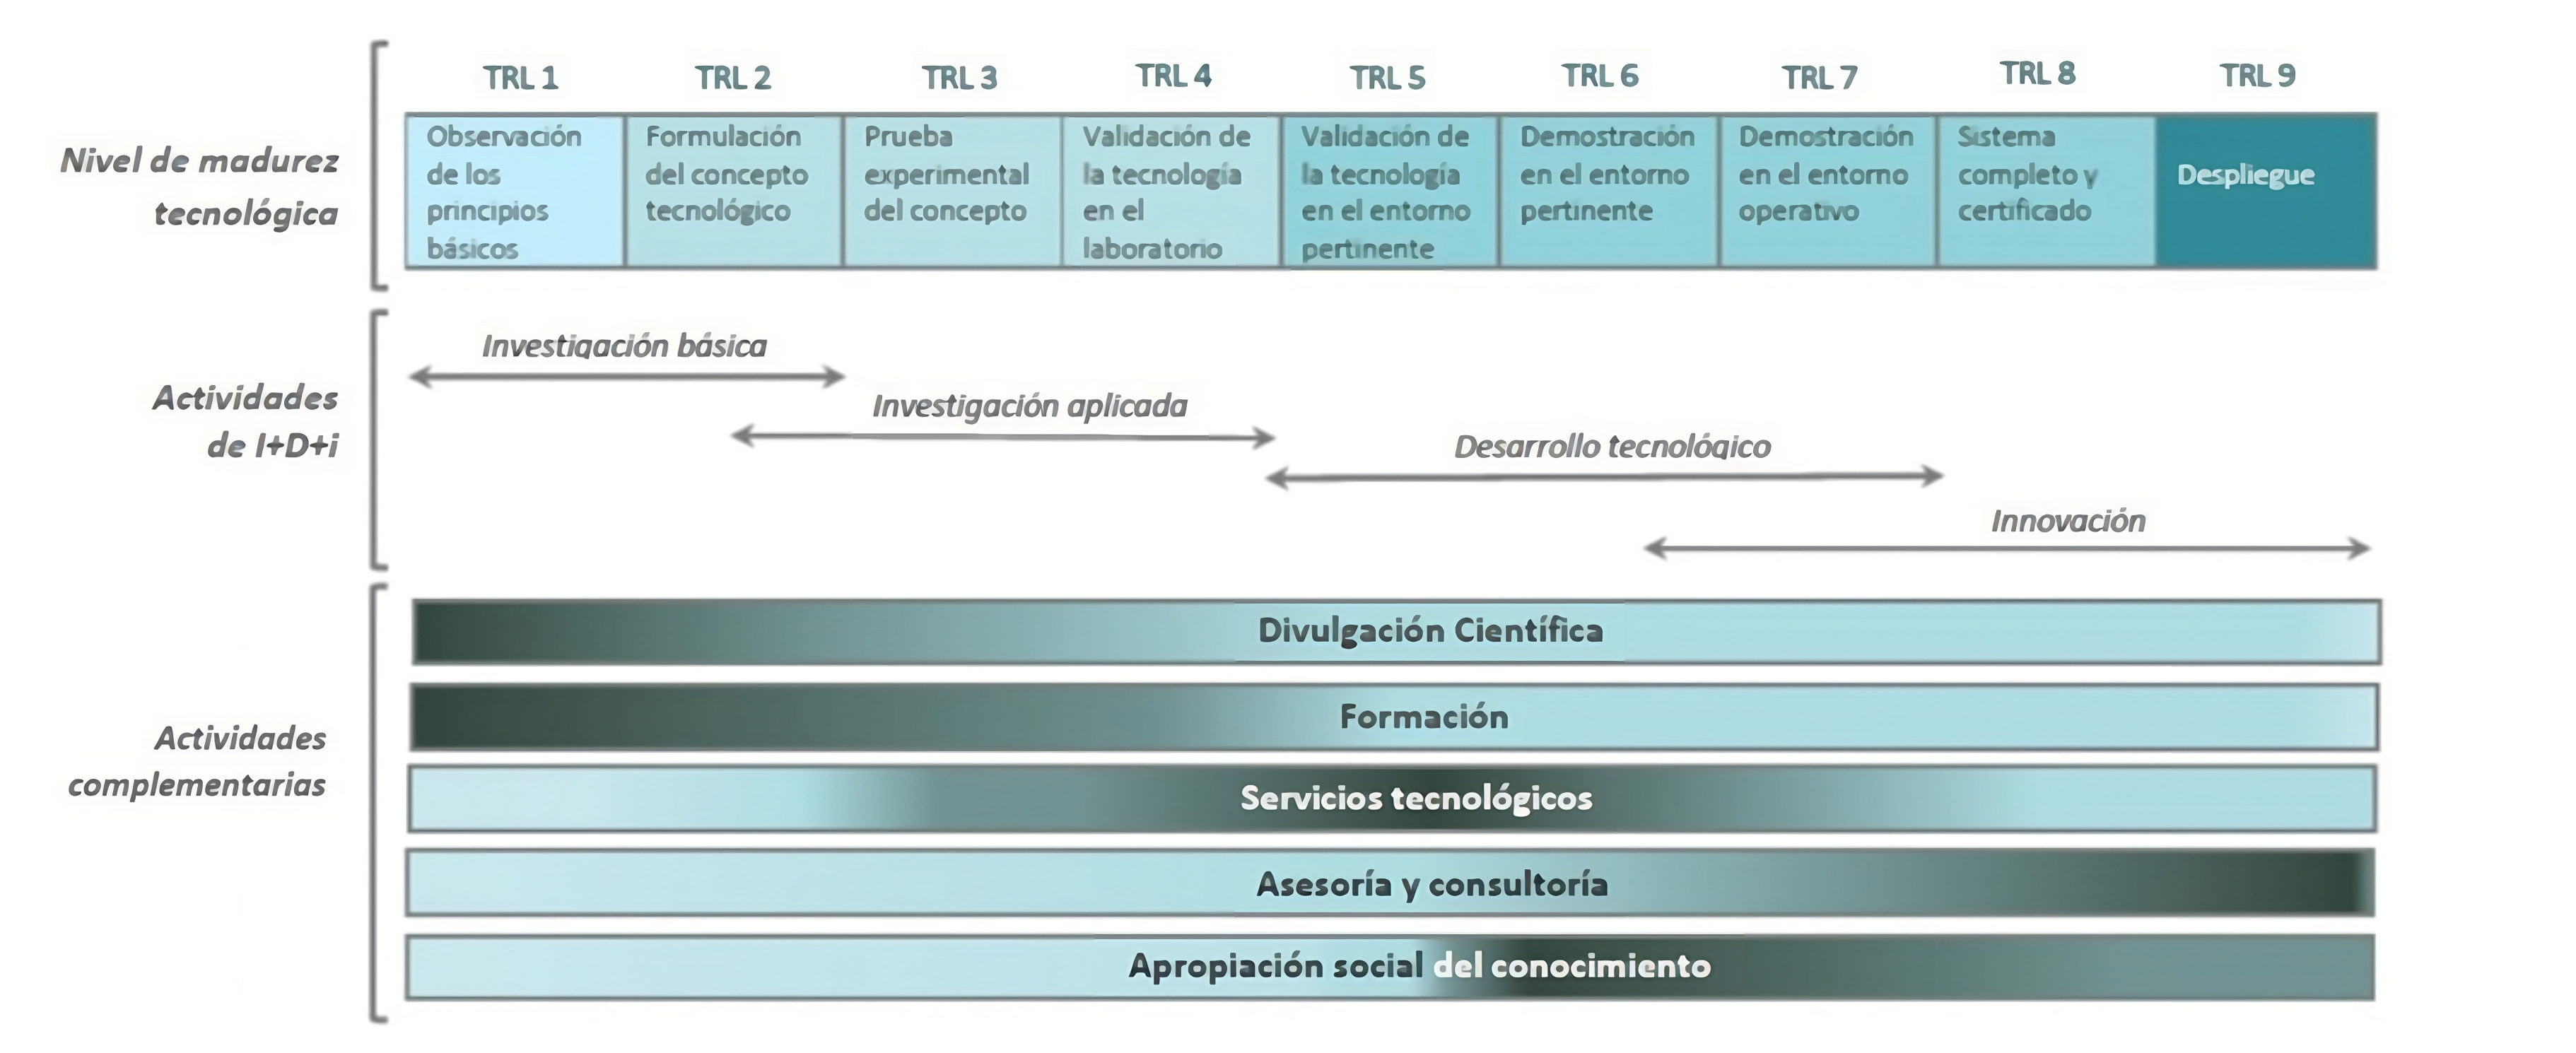
\includegraphics[width=1\linewidth]{Imagenes/Niveles_de_maduracion_tecnologica-transformed (1).png}
    \caption{Niveles de TLR Colciencias}
    Fuente: Colciencias \cite{colciencias2018trl}
    \label{fig:tlr}
\end{figure}
Como se muestra en la Figura \ref{fig:tlr}, existen 9 niveles de maduración tecnológica (TRL)  los cuales comprenden el ciclo de maduración de un proyecto y/o investigación [20], pasando por una investigación básica, investigación aplicada, desarrollo tecnológico y por último innovación. El presente proyecto se encuentra entre el nivel de TRL 5 y TRL 6, pues en estos 2 niveles se realiza la validación del proyecto para su entorno objetivo, lo cual se aplicó en el capitulo 7 mediante las encuestas realizadas.